\chapter{TaCとTacOS}
\label{TacAndTacOS}
TaC(Tokuyama Advanced educational Computer)は,
TeC7(Tokuyama Educational Computer Ver.7)\footnote{
  詳細は\url{https://github.com/tctsigemura/TeC7}を参照のこと.}に内蔵された
16bitのコンピュータである.
TeC7基板上のジャンパ設定によりTaCモードに切り換える.
\figref{tacPhoto}に写真を示す.
TaCは,ディスプレイ,キーボード,マイクロSDカードを接続することで,
1980年代前半の8bitパソコン程度の能力を発揮する.
コンピュータサイエンスを学ぶ大学や高専の学生が,
実際に動作するPCの例として使用したり,
仕組みを解析する目的で設計してある.

\begin{myfig}{btp}{TeC7とTaC}{tacPhoto}
  \begin{minipage}{0.58\columnwidth}
    \begin{center}
      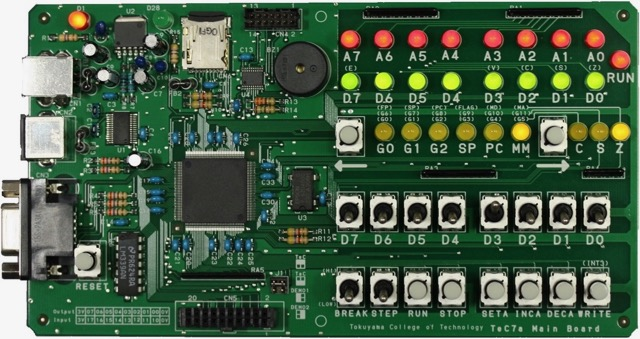
\includegraphics[scale=0.35]{Photo/TeC7.jpg}\\
      \subcaption{TeC7の写真}
      \label{fig:tec7Photo}
    \end{center}
  \end{minipage}
  \begin{minipage}{0.38\columnwidth}
    \begin{center}
      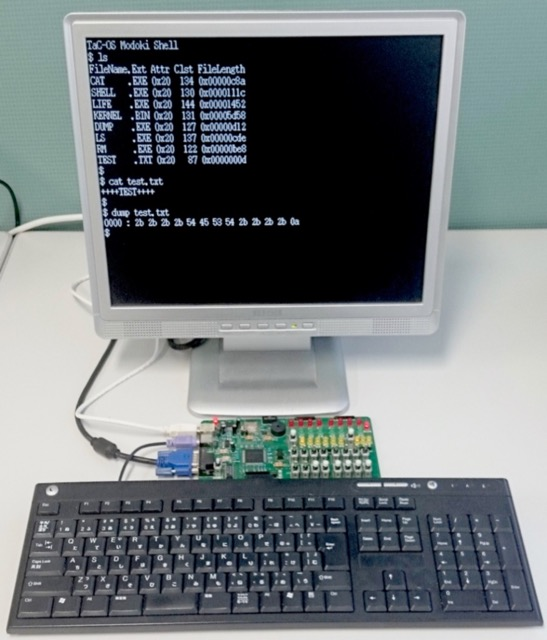
\includegraphics[scale=0.29]{Photo/TaC.jpg}\\
      \subcaption{TaCとしての使用例}
    \end{center}
  \end{minipage}
\end{myfig}

TaC上では{\cmml}\footnote{
  C言語に似た言語,
  詳細は\url{https://github.com/tctsigemura/C--/blob/master/doc/cmm.pdf}を
  参照のこと.}で記述されたTacOS\footnote{
  詳細は\url{https://github.com/tctsigemura/TacOS}を参照のこと.} が動作する.
本書ではTacOSをオペレーティングシステムの実装例として参照する.

%==============================================================================
\section{ハードウェア構成}
\figref{tacBlock}にTaCのハードウェア構成を示す.
16ビットのシングルプロセッサ(CPUが一つ),
主記憶64KiBの非常に単純なシステムである.
単純なのでオペレーティングシステムの構築も容易である.
TaCに関する資料を付録\ref{appTac}にまとめる.

\begin{myfig}{btp}{TaCのハードウェア構成}{tacBlock}
  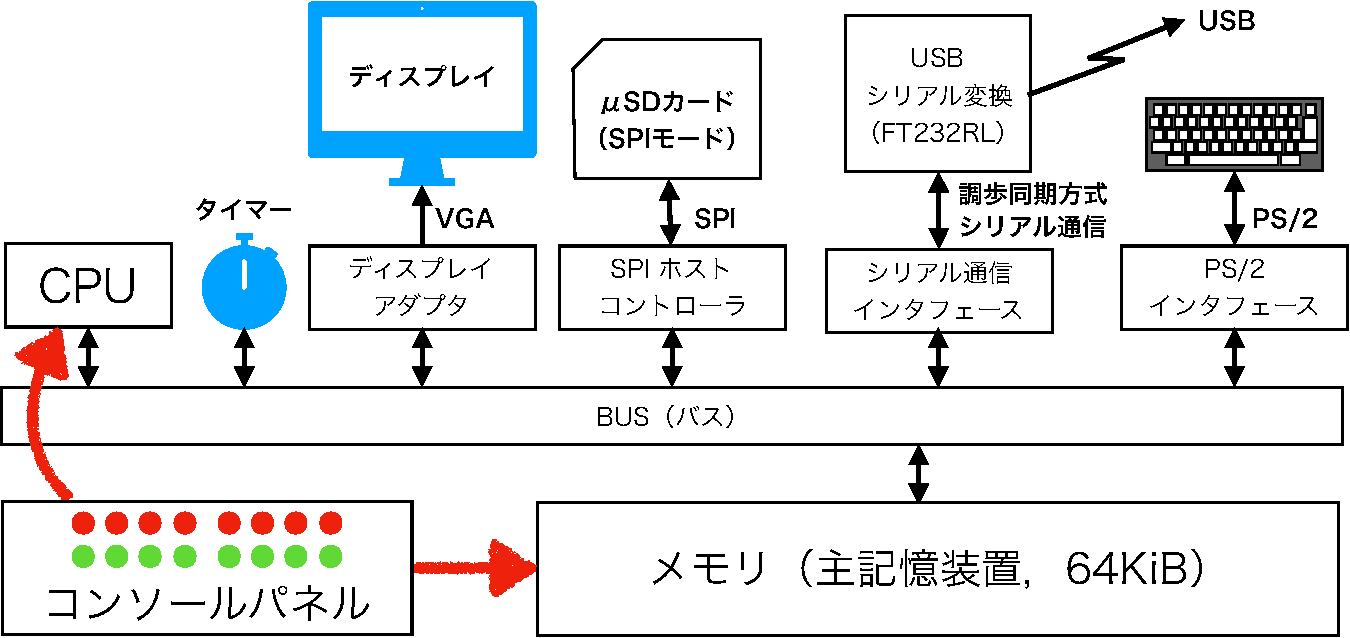
\includegraphics[scale=0.55]{Fig/tacBlock-crop.pdf}
\end{myfig}

\begin{itemize}
\item \emph{コンソールパネル} \\
  \figref{tec7Photo}で,
  TeC7本体右半分のランプやスイッチで構成される部分をコンソールパネルと呼ぶ.
  コンソールパネルはCPUや主記憶と直接接続されており,
  CPUを停止した状態で,
  CPUや主記憶の内容を操作したり観察したりすることができる.
  また,機械語命令を一命令毎に実行するステップ実行機能や,
  ある番地の命令を実行した時点でプログラムを停止する
  ブレークポイント機能が利用できる.
  コンソールパネルの機能はハードウェアで実現されているので,
  オペレーティングシステムの内部をステップ実行することも可能である.
  TacOSの開発では,コンソールパネルがデバッグに活用された.
\item \emph{CPU} \\
  \figref{tacRegPsw}に示すようなCPUレジスタとPSWを持つ16ビットCPUである.
  PSWのフラグに実行モードを表すPビットを持ち,
  カーネルモードとユーザモードを切り換えることができる.
  機械語命令は,\figref{tacInsTbl}に示す46種類が準備されている.
  機械語命令のアドレッシングモードは8種類ある.
\item \emph{メモリ} \\
  メモリは\figref{tacMap}に示す構成である.
  メモリ空間全体で64KiB,
  自由に使用できるメモリが56KiB,
  2KiBのVRAMと4KiBのIPL,32Bの割込みベクタからなる.
  メモリは8ビット単位,または,16ビット単位で読み書きできる.
  16ビット単位の場合は偶数アドレスを用いる.
\item \emph{タイマー} \\
  $1$ミリ秒から$2^{16}-1$ミリ秒までの間隔で割込みを発生する
  二つのインターバルタイマーが利用できる.
\item \emph{ディスプレイアダプタ} \\
  80文字×24行の文字をVGAディスプレイに表示する.
  メモリ空間の\|E000h|から配置されるVRAMに書き込んだ
  ASCIIコードと対応する文字をディスプレイに表示する.
  \|E000h|番地がディスプレイの左上隅に対応する,
  \|E001h|番地が一行目の2文字の位置,
  \|E04Fh|番地が一行目の80文字の位置,
  \|E050h|番地が二行目の1文字の位置に対応する.
\item \emph{SPIホストコントローラ} \\
  スロットに挿入されたマイクロSDカードをSPIモードに切換え読み書きを行う.
  SPIホストコントローラに初期化コマンドを発行すると,
  マイクロSDカードをSPIモードに切換える.
  ブロックアドレスとメモリアドレスを設定して読み出しコマンドを発行すると,
  マイクロSDカードの指定したブロックから512バイトのデータを
  CPUを介さずに(DMA:Direct Memory Accessを用いて)メモリに読み出す.
  書込みコマンドを発行すると,
  メモリから指定ブロックにデータを書き込む.
\item \emph{シリアル通信インタフェース} \\
  調歩同期方式,9,600Baudの通信インタフェースである.
  USBシリアル変換ICを通してPC等のシリアルターミナルと通信できる.
  1バイト転送する毎に割込みを発生する.
\end{itemize}

%==============================================================================
\section{TacOS}
\begin{myfig}{btp}{TacOSの構成}{tacosOrganization}
  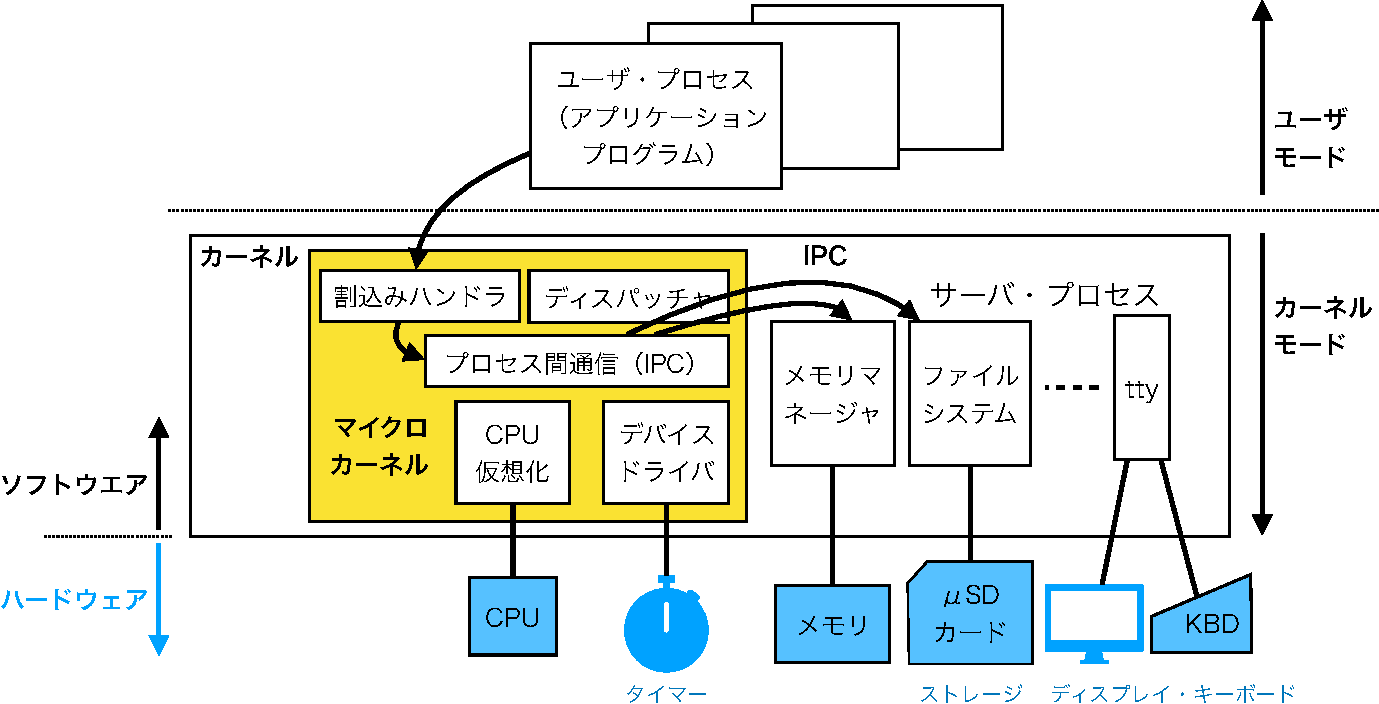
\includegraphics[scale=0.66]{Fig/tacosOrganization-crop.pdf}
\end{myfig}

\figref{tacosOrganization}にTaC用のOSであるTacOSの構造を示す.
マイクロカーネルがプロセス間通信(IPC)機能を提供し,
サーバプロセスがメモリ管理やファイルシステム機能を提供する.
\figref{microkernel}の一般的なマイクロカーネル方式と異なり,
サーバプロセスがカーネルモードで動作しハードウェアに直接アクセスする.
また,サーバプロセスはマイクロカーネルとリンクされ一つの
プログラムモジュールになる.
このプログラムモジュールを\emph{カーネル}と呼ぶことにする.
同じプログラムモジュール内なので,サーバプロセスは
マイクロカーネル内ルーチンをCALL機械語命令で直接に呼び出すことができる.

割込みやSVC命令の実行が原因で,
ユーザプロセスはカーネルモードに切り換わり
マイクロカーネル内の割込みハンドラが呼び出される.
割込みハンドラで割込み原因を判断し,
マイクロカーネル内のルーチンを呼び出したり,
サーバプロセスの機能をIPCを用いて呼び出したりする.

%==============================================================================
\section{まとめ}
\emph{TaC}は,本書でオペレーティングシステムの実装例として使用する
TacOSを稼働させるコンピュータである.
コンソールパネルを持ち,
TacOSのカーネル内までステップ実行によるトレースが可能である.
\emph{TacOS}はマイクロカーネル方式の簡単なオペレーティングシステムである.
本書では,しばしばTacOSのソースコードを実装例として参照する.
